\Section{Move Prover Design}

\begin{Figure}
  \centering
  \caption{Move Prover Architecture}
  \label{fig:Arch}
  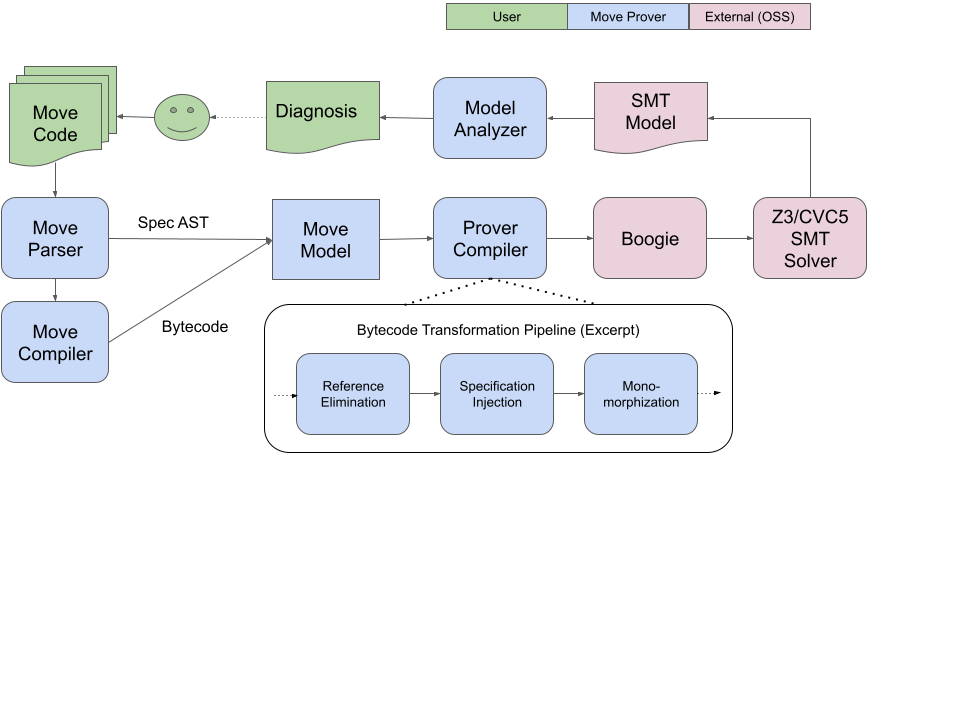
\includegraphics[trim=0 250 0 0, width=\textwidth]{arch.png}
\end{Figure}

The architecture of \MVP is illustrated in Fig.~\ref{fig:Arch}. Move code
(containing specifications) is given as input to the tool chain, which
produces two artifacts: an abstract syntax tree (AST) of the specifications,
and the generated bytecode.  The \emph{Move Model} merges both bytecode and
specifications, as well as other metadata from the original code, into a
unified object model which is input to the remaining tool chain.

The next phase is the actual \emph{Prover Compiler}, which is a
pipeline of bytecode transformations. We focus on the
transformations shown (Reference Elimination, Specification Injection, and
Monomorphization).
%% These transformations will be conceptually described in more
%% detail in subsequent sections.
The Prover uses a modified version of the Move VM bytecode as an intermediate
representation for these transformations, but, for clarity,
we describe the transformations at the Move source level.

The transformed bytecode is next compiled into the Boogie intermediate
verification language \cite{BOOGIE}. Boogie supports an imperative programming
model which is well suited for the encoding of the transformed Move code. Boogie
in turn can translate to multiple SMT solver backends, namely Z3 \cite{Z3} and
CVC5 \cite{CVC}; the default choice for the Move prover is currently Z3.

% When the SMT solver produces a |sat| or |unknown| result (of the negation of the
% verification condition Boogie generates), it produces a model witness. The Move
% Prover attempts to translate this model back into a diagnostic which
% a user can associate with the original Move code (as has been illustrated in
% Sec.~\ref{sec:RunningProver}.) For example, execution traces leading to the
% verification failure are shown, with assignments to variables used in this
% trace, extracted from the model. Also the Move Model will be consulted to
% retrieve the original source information and display it with the diagnosis.

%% Subsequently, we will focus on the major bytecode transformations.

\SubSection{Reference Elimination}
\label{sec:RefElim}

The reference elimination transformation is what enables the
alias-free memory model in the Move Prover, which is one of the most
important factors contributing to the speed and reliability of the
system.  In most software verification and static analysis systems,
the explosion in number of possible aliasing relationships between
references leads either to high computational complexity or harsh
approximations.

In Move, the reference system is based on
\emph{borrow semantics}~\cite{BORROW_SEM} as in the Rust programming language.
%
The initial borrow must come from either
a global memory or
a local variable on stack
(both referred to as \emph{locations} from now on).
%
For local variables, one can create
immutable references (with syntax |&x|) and
mutable references (with syntax |&mut x|).
%
For global memories, the references can be created via the
|borrow_global| and |borrow_global_mut| built-ins.
%
Given a reference to a whole struct,
field borrowing can occur via |&mut x.f| and |&x.f|.
%
Similarly, with a reference to a vector,
element borrowing occurs via native functions
|Vector::borrow(v, i)| and |Vector::borrow_mut(v, i)|.
%
Move provides the following guarantees,
which are enforced by the borrow checker:
% ~\cite{BORROW_CHECKER}:

\begin{itemize}
\item For any location, there can be
  either exactly one mutable reference,
  or $n$ immutable references.
  %
  Enforcing this rule is similar to enforcing the borrow semantics
  in Rust, except for global memories, which do not exist in Rust.
  %
  For global memories,
  this rule is enforced via the |acquires| annotations.
  %
  Using Fig.~\ref{fig:AccountDef} as an example,
  function |withdraw| |acquires| the |Account| global location,
  therefore, |withdraw| is prohibited from calling any other function that might
  also borrow or modify the |Account| global memory (e.g., |deposit|).
\item The lifetime of references to data on the stack
  cannot exceed the lifetime of the stack location.
  %
  This includes global memories borrowed inside a function as well---a
  reference to a global memory cannot be returned from the function,
  neither in whole nor in parts.
\end{itemize}

\noindent These properties effectively permit the \emph{elimination of
  references} from a Move program, eliminating need to reason about aliasing.

\Paragraph{Immutable References}

Immutable references are replaced by values.
An example of the applied transformation is shown below. We remove the reference
type constructor and all reference-taking operations from the code:

\begin{Move}
  fun select_f(s: &S): &T { &s.f } @\transform@ fun select_f(s: S): T { s.f }
\end{Move}

\noindent
When executing a Move program, immutable references are important to avoid copies
for performance and to enforce ownership; however, for symbolic reasoning on
correct Move programs, the distinction between immutable references and values
is unimportant.

\Paragraph{Mutable References}
\label{sec:RefElimMut}

Each mutation of a location |l| starts with an initial borrow for the whole data
stored in this location. This borrow creates a reference |r|.
%
As long as |r| is alive, Move code can either update its value (|*r = v|),
or derive a sub-reference (|r' = &mut r.f|).
%
The mutation ends when |r| (and the derived |r'|) go out of scope.

The borrow checker guarantees that during the mutation
of the data in |l|, no other reference can exist into the same data in |l|
-- meaning that it is impossible for other Move code to test whether the
value has mutated while the reference is held.

%% The fact that |&mut| has exclusive access to the whole value in a location
These semantics allow mutable references to be handled via
\emph{read-update-write} cycles.
%
One can create a copy of the data in |l| and
perform a sequence of mutation steps which are represented as purely functional
data updates.
%
Once the last reference for the data in |l| goes out of scope, the updated value
is written back to |l|.
%
This
%% effectively turns
converts an imperative program with references
into an imperative program which only has state updates on global memory or
variables on the stack,
%% a class of programs which is known to have a significantly
%% simpler semantics.
with no aliasing.
We illustrate the basics of this approach by an example:

\begin{Move}
  fun increment(x: &mut u64) { *x = *x + 1 }
  fun increment_field(s: &mut S) { increment(&mut s.f) }
  fun caller(): S { let s = S{f:0}; update(&mut s); s }
  @\transform@
  fun increment(x: u64): u64 { x + 1 }
  fun increment_field(s: S): S { s[f = increment(s.f)] }
  fun caller(): S { let s = S{f:0}; s = update(s); s }
\end{Move}

\Paragraph{Dynamic Mutable References}

While the setup in above example covers a majority of the use cases in every day
Move code,
%% there are more complex ones to consider, namely that the value of a
%% reference depends on runtime decisions.
the general case is more complex, since the referenced location may not be known
statically.
Consider the following Move code:

\begin{Move}
  let r = if (p) &mut s1 else &mut s2;
  increment_field(r);
\end{Move}

\noindent Additional information in the logical encoding is required to deal
with such cases.
%% At the execution point
When a reference goes out of scope, we need to know
from which location it was derived in order to write back the updated value.
%
Fig.~\ref{fig:MutElim} illustrates the approach for doing this.
%
Essentially, a new type |Mut<T>|, which is internal to \MVP, is introduced to
track both the location from which |T| was derived and the value of |T|.
%
|Mut<T>| supports the following operations:

\begin{itemize}
\item |Mvp::mklocal(value, LOCAL_ID)| creates a new mutation value for a local
  with the given local id.  A local id uniquely identifies a local variable
  in the function.
\item Similarly, |Mvp::mkglobal(value, TYPE_ID, addr)| creates a new
  mutation for a global with given type and address.
  %% DD: Guessing readers won't care about this detail. Or we can drop the address.
  %% Notice that in the
  %%   current Move type system, we would not need to represent the address, since
  %%   there can be only one mutable reference into the entire type (via the
  %%   acquires mechanism). However, we keep this more general here, as the Move
  %%   type system might change.
\item With |r' = Mvp::field(r, FIELD_ID)| a mutation value for a sub-reference is
  created for the identified field.
\item The value of a mutation is replaced with |r' = Mvp::set(r, v)| and
  retrieved with |v = Mvp::get(r)|.
\item With the predicate |Mvp::is_local(r, LOCAL_ID)| one can test whether |r|
  was derived from the given local, and with |Mvp::is_global(r, TYPE_ID, addr)|
  for a specific global location.~%
  |Mvp::is_field(r, FIELD_ID)| tests whether |r| is derived from the given field.
\end{itemize}

\begin{figure}[t!]
  \caption{Elimination of Mutable References}
  \label{fig:MutElim}
  \centering
\begin{MoveBoxNumbered}
  fun increment(x: &mut u64) { *x = *x + 1 }
  fun increment_field(s: &mut S) {
    let r = if (s.f > 0) &mut s.f else &mut s.g;
    increment(r)
  }
  fun caller(p: bool): (S, S) {
    let s1 = S{f:0, g:0}; let s2 = S{f:1, g:1};
    let r = if (p) &mut s1 else &mut s2;
    increment_field(r);
    (s1, s2)
  }
  @\transform@
  fun increment(x: Mut<u64>): Mut<u64> { Mvp::set(x, Mvp::get(x) + 1) }
  fun increment_field(s: Mut<S>): Mut<S> {
    let r = if (s.f > 0) Mvp::field(s.f, S_F) else Mvp::field(s.g, S_G);
    r = increment(r);
    if (Mvp::is_field(r, S_F))
      s = Mvp::set(s, Mvp::get(s)[f = Mvp::get(r)]);
    if (Mvp::is_field(r, S_G))
      s = Mvp::set(s, Mvp::get(s)[g = Mvp::get(r)]);
    s
  }
  fun caller(p: bool): S {
    let s1 = S{f:0, g:0}; let s2 = S{f:1, g:1};
    let r = if (p) Mvp::mklocal(s1, CALLER_s1)
            else Mvp::mklocal(s2, CALLER_s2);
    r = increment_field(r);
    if (Mvp::is_local(r, CALLER_s1))
      s1 = Mvp::get(r); @\label{line:WriteBack}@
    if (Mvp::is_local(r, CALLER_s2))
      s2 = Mvp::get(r);
    (s1, s2)
  }
\end{MoveBoxNumbered}
\end{figure}

\MVP implements the illustrated transformation by construction a \emph{borrow
  graph} from the program via data flow analysis.  This graph tracks both when
references are released as well as how they relate to each other: e.g.~%
|r' = &mut r.f| creates an edge from |r| to |r'| labeled with |f|, and~%
|r' = &mut r.g| creates another also starting from |r|.  The borrow analysis is
inter-procedural, requiring computed summaries for the borrow graph of called
functions.

The resulting borrow graph is then used to guide the transformation, inserting
the operations of the |Mut<T>| type as illustrated in
Fig~\ref{fig:MutElim}. Specifically, when the borrow on a reference ends, the
associated mutation value must be written back to its parent mutation or the
original location (e.g. line~\ref{line:WriteBack} in
Fig.~\ref{fig:MutElim}). The presence of multiple possible origins leads to case
distinctions via |Mvp::is_X| predicates; however, these cases are rare in actual
Move programs.


\SubSection{Global Invariant Injection}
\label{sec:GlobalInvariants}

Correctness of smart contracts is largely about the correctness of the
blockchain state, so global invariants are particular important in the
move specification language.  For example, in the Diem framework,
global invariants can capture the requirement that an account be
accompanied by various other types that are be stored at the same
address and the requirement certain state changes are only permitted
for certain accounts by the access control scheme.

Most software verification tools prove that functions preserve
invariants by assuming the invariant at the entry to each function and
proving them at the exit.  In a module or class, it is only necessary
to prove that invariants are preserved by public functions, since
invariants are often violated internally in the implementation of a module or
class. An earlier version of the Move Prover used exactly this approach.

The current implementation of the Prover takes the opposite approach: it ensures
that invariants hold after every instruction, unless explicitly directed to
suspend some invariants by a user.  This \emph{fine-grained} approach has
performance advantages, because, unless suspended, \emph{invariants are only
  proven when an instruction is executed that could invalidate them}, and the
proofs are often computationally simple because \emph{the change from a single
  instruction is usually small}.  Relatively few invariants are suspended, and,
when they are, it is over a relatively small span of instructions, preserving
these advantages.  There is another important advantage, which is that
invariants hold almost everywhere in the code, so they are available to approve
other properties, such as abort conditions. For example, if a function accesses
type |T1| and then type |T2|, the access to |T2| will never abort if the
presence of |T1| implies the presence of |T2| at every state in the body of the
function.  This situation occurs with some frequency in the Diem framework.


\Paragraph{Invariant Types and Proof Methodology}

\emph{Inductive} invariants are properties declared in Move modules that must
(by default) hold for the global memory at all times. Those invariants often
quantify over addresses (See Fig.~\ref{fig:AccountSpec} for example.) Based on
Move's borrow semantics, inductive invariants don't need to hold while memory is
mutated because the changes are not visible to other code until the change is written back.
This is reflected by the reference elimination described in
Sec.~\ref{sec:RefElim},

\emph{Update} invariants are properties that relate two states, a previous state
and the current state.  Typically they are enforced after an update of global
memory. The |old| operator is used to evaluate specification expressions in the
previous state.

Verification of both kinds of invariants can be \emph{suspended}. That means,
instead of being verified at the time a memory update happens, they are verified
at the call site of the function which updates memory. This feature is
necessitated by fine-grained invariant checking, because invariants sometimes do
not hold in the midst of internal computations of a module. For example, a
relationship between state variables may not hold when the variables are being
updated sequentially.  Functions with external callers (public or script
functions) cannot suspend invariant verification, since the invariants are
assumed to hold at the beginning and end of each such function.


Inductive invariants are proven by induction over the evolution of the global
memory. The base case is that the invariant must hold in the empty state that
precedes the genesis transaction.  For the induction step, we can assume that
the invariant holds at each verified function entry point for which it is not
suspended, and now must prove that it holds after program points which are
either direct updates of global memory, or calls to functions which suspend
invariants.

For update invariants, no induction proof is needed, since they just relate two
memories.  The pre-state is some memory captured before an update happens, and
the post state the current state.

\Paragraph{Modular Verification}

We wish to support open systems to which untrusted modules can be added
with no chance of violating invariants that have already been proven. For each
invariant, there is a defined subset of Move modules (called a
\textit{cluster}). If the invariant is proven for the modules in the cluster, it
is guaranteed to hold in all other modules -- even those that were not yet
defined when the invariant was proven.  The cluster must contain every function
that can invalidate the invariant, and, in case of invariant suspension, all
callers of such a function.  Importantly, functions outside the cluster can
never invalidate an invariant. Those functions trivially preserve the
invariant, so it is only necessary to verify functions defined in the cluster.

% \TODO{Dave}{Is the next paragraph accurate? My original plan was that
%   there would be one target module, we would verify its invariants,
%   and would pull in dependencies, friends of dependencies, and
%   dependencies of friends (I think we don't need the dependencies of
%   friends).  Some subset of the functions in this set would be
%   instrumented.  It isn't the SMALLEST set of functions or modules --
%   but it includes (at least) all of the clusters for all of the invariants.}

\MVP verifies a given set of modules at a time (typically one).  The modules
being verified are called the \textit{target modules}, and the global invariants
to be verified are called \textit{target invariants}, which are all invariants
defined in the target modules. The cluster is then the smallest set as specified
above such that all target modules are contained.

\Paragraph{Basic Translation}

\begin{Figure}
  \caption{Basic Global Invariant Injection}
  \label{fig:GlobalInvariants}
  \centering
\begin{MoveBox}
  fun f(a: address) {
    let r = borrow_global_mut<S>(a);
    r.value = r.value + 1
  }
  invariant [I1] forall a: address: global<S>(a).value > 0;
  invariant [I2] update forall a: address:
      global<S>(a).value > old(global<S>(a).value);
  @\transform@
  fun f(a: address) {
    spec assume I1;
    Mvp::snapshot_state(I2_BEFORE);
    r = <increment mutation>;
    spec assert I1;
    spec assert I2[old = I2_BEFORE];
  }
\end{MoveBox}
\end{Figure}


We first look at injection of global invariants in the absence of
% memory and functions with
type parameters. Fig.~\ref{fig:GlobalInvariants} contains an
example for the supported invariant types and their injection into code. The
first invariant, |I1|, is an inductive invariant. It is assumed on function
entry, and asserted after the state update. The second, |I2|, is an update
invariant, which relates pre and post states. For this a state snapshot is
stored under some label |I2_BEFORE|, which is then used in an assertion.

Global invariant injection is optimized by knowledge of the prover, obtained by
static analysis, about accessed and modified memory.  Let |accessed(f)| be the
memory accessed by a function, and |modified(f)| be the memory modified. Let
|accessed(I)| by an invariant (including transitively by all functions it
calls).

\begin{itemize}
\item Inject |assume I| at entry to |f| \emph{if} |accessed(f)| has overlap with
  |accessed(I)|.
\item Inject |assert I| after each program step if one of the following is true
  (a) the step modifies a memory location |M in accessed(I)| or, (b) the step is
  a call to function |f'| in which |I| is suspended and |modifies(f')|
  intersects with |accessed(I)|.  Also, if |I| is an update invariant, inject a
  save of a memory snaptshot before the update or call.
\end{itemize}

\vspace{-1ex}
\Paragraph{Genericity}

\begin{Figure}
  \caption{Global Invariant Injection and Genericity}
  \label{fig:Genericity}
  \centering
\begin{MoveBox}
  invariant [I1] global<S<u64>>(0).value > 1;
  invariant<T> [I2] global<S<T>>(0).value > 0;
  fun f(a: address) { borrow_global_mut<S<u8>>(0).value = 2 }
  fun g<R>(a: address) { borrow_global_mut<S<R>>(0).value = 3 }
  @\transform@
  fun f(a: address) {
    spec assume I2[T = u8];
    <<mutate>>
    spec assert I2[T = u8];
  }
  fun g<R>(a: address) {
    spec assume I1; spec assume I2[T = R];
    <<mutate>>
    spec assert I1; spec assert I2[T = R];
  }
\end{MoveBox}
\end{Figure}

Generic type parameters make the problem of determining whether a function can
modify an invariant more difficult.  Consider the example in
Fig.~\ref{fig:Genericity}. Invariant |I1| holds for a specific type
instantiation |S<u64>|, whereas |I2| is generic over all type instantiations for
|S<T>|.

The non-generic function |f| which works on the instantiation |S<u8>| will have
to inject the \emph{specialized} instance |I2[T = u8]|. The invariant |I1|,
however, does not apply for this function, because there is no overlap with
|S<u64>|.  In contrast, |g| is generic in type |R|, which could be instantiated
to |u64|. So, |I1|, which applies to |S<u64>| needs to be injected
in addition to |I2|.
%% relevant for the specific case of |S<u64>|.

The general solution depends on type unification.  Given the accessed memory of
a function |f<R>| and an invariant |I<T>|, we compute the pairwise unification
of memory types. Those types are parameterized over |R| resp. |T|. Successful
unification results in a substitution for both type parameters, and we include
the invariant with |T| specialized according to the substitution.

\SubSection{Monomorphization}
\label{sec:Mono}

Monomorphization is a transformation which removes generic types from a Move
program by \emph{specializing} the program for relevant type instantiations.  In
the context of verification, the goal is that the specialized program verifies
if and only if the generic program verifies in an encoding which supports types
as first class values. We expect the specialized program to verify faster
because it avoids the problem of generic representation of values, supporting
a multi-sorted representation in the SMT logic.


\begin{Figure}
\caption{Basic Monomorphization}
\label{fig:Mono}
\centering
\begin{MoveBox}
  struct S<T> { .. }
  fun f<T>(x: T) { g<S<T>>(S(x)) }
  fun g<S:key>(s: S) { move_to<S>(.., s) }
  @\transform@
  struct T{}
  struct S_T{ .. }
  fun f_T(x: T) { g_S_T(S_T(x)) }
  fun g_S_T(s: S_T) { move_to<S_T>(.., s) }
\end{MoveBox}
\end{Figure}

To verify a generic function for all possible instantiations, monomorphization
skolemizes the type parameter, i.e.~the function is verified for a new type
with no special properties that represents an arbitrary type.  It then
specializes all called functions and used data types with this new type and any
other concrete types they may use.  Fig.~\ref{fig:Mono} sketches this approach.

However, this approach has one issue: the type of genericity Move provides does
not allow for full type erasure (unlike many programming languages) because
types are used to \emph{index} global memory (e.g. |global<S<T>>(addr)| where
|T| is a generic type). Consider the following Move function:

\begin{Move}
  fun f<T>(..) { move_to<S<T>>(s, ..); move_to<S<u64>>(s, ..) }
\end{Move}

\noindent Depending on how |T| is instantiated, this function behaves
differently.  Specifically, if |T| is instantiated with |u64| the function will
always abort at the second |move_to|, since the target location is already
occupied.

The important property enabling monomorphization in the presence of such type
dependent code is that one can identify the situation by looking at the memory
accessed by code and injected specifications. From this one can derive
\emph{additional instantiations of the function} which need to be verified. In
the example above, verifying both |f_T| and an instantiation |f_u64| will cover
all relevant cases of the function behavior.

The algorithm for computing the instances that require verification works as
follows. Let |f<T1,..,Tn>| be a verified target function which has all
specifications injected and inlined function calls expanded.
\begin{itemize}
\item For each memory~~|M in modified(f)|, if there is a memory~%
  |M' in modified(f) + accessed(f)| such that |M| and |M'| can unify via
  |T1,..,Tn|, collect an instantiation of the type parameters |Ti| from the
  resulting substitution. This instantiation may not assign values to all type
  parameters, and those unassigned parameters stay as is. For instance,~%
  |f<T1, T2>| might have a partial instantiation |f<T1, u8>|.
\item Once all partial instantiations are computed, the set is
  extended by unifying the instantiations against each other. If |<T>| and
  |<T'>| are in the set, and they unify under the substitution |s|, then
  |<s(T)>| will also be part of the set.  For example, consider |f<T1, T2>|
  which modifies |M<T1>| and |R<T2>|, as well as accesses |M<u64>| and
  |R<u8>|. From this the instantiations |<u64, T2>| and |<T1, u8>| are computed,
  and the additional instantiation |<u64, u8>| will be added to the set.
\item If after computing and extending instantiations any type parameters
  remain, they are skolemized into a given type as described earlier.
\end{itemize}

\noindent To understand the correctness of this procedure, consider the
following arguments (a full formal proof is outstanding):

\begin{itemize}
\item \emph{Direct interaction} Whenever a modified memory |M<t>| can influence
  the interpretation of |M<t'>|, a unifier must exist for the types |t| and |t'|,
  and an instantiation will be verified which covers the overlap of |t| and
  |t'|.
\item \emph{Indirect interaction} If there is an overlap between two types
  which influences whether another overlap is semantically relevant, the
  combination of both overlaps will be verified via the extension step.
\end{itemize}

Notice that even though it is not common in regular Move code to work with both
memory |S<T>| and, say, |S<u64>| in one function, there is a scenario where such
code is implicitly created by injection of global invariants. Consider the
example in Fig.~\ref{fig:Genericity}. The invariant |I1| which works on |S<u64>|
is injected into the function |g<R>| which works on |S<R>|. When monomorphizing
|g|, we need to verify an instance |g_u64| in order to ensure that |I1| holds.



%%% Local Variables:
%%% mode: latex
%%% TeX-master: "main"
%%% End:
